% Options for packages loaded elsewhere
\PassOptionsToPackage{unicode}{hyperref}
\PassOptionsToPackage{hyphens}{url}
%
\documentclass[
]{article}
\title{Social Norms Meta-Analysis Information}
\author{}
\date{\vspace{-2.5em}}

\usepackage{amsmath,amssymb}
\usepackage{lmodern}
\usepackage{iftex}
\ifPDFTeX
  \usepackage[T1]{fontenc}
  \usepackage[utf8]{inputenc}
  \usepackage{textcomp} % provide euro and other symbols
\else % if luatex or xetex
  \usepackage{unicode-math}
  \defaultfontfeatures{Scale=MatchLowercase}
  \defaultfontfeatures[\rmfamily]{Ligatures=TeX,Scale=1}
\fi
% Use upquote if available, for straight quotes in verbatim environments
\IfFileExists{upquote.sty}{\usepackage{upquote}}{}
\IfFileExists{microtype.sty}{% use microtype if available
  \usepackage[]{microtype}
  \UseMicrotypeSet[protrusion]{basicmath} % disable protrusion for tt fonts
}{}
\makeatletter
\@ifundefined{KOMAClassName}{% if non-KOMA class
  \IfFileExists{parskip.sty}{%
    \usepackage{parskip}
  }{% else
    \setlength{\parindent}{0pt}
    \setlength{\parskip}{6pt plus 2pt minus 1pt}}
}{% if KOMA class
  \KOMAoptions{parskip=half}}
\makeatother
\usepackage{xcolor}
\IfFileExists{xurl.sty}{\usepackage{xurl}}{} % add URL line breaks if available
\IfFileExists{bookmark.sty}{\usepackage{bookmark}}{\usepackage{hyperref}}
\hypersetup{
  pdftitle={Social Norms Meta-Analysis Information},
  hidelinks,
  pdfcreator={LaTeX via pandoc}}
\urlstyle{same} % disable monospaced font for URLs
\usepackage[margin=1in]{geometry}
\usepackage{graphicx}
\makeatletter
\def\maxwidth{\ifdim\Gin@nat@width>\linewidth\linewidth\else\Gin@nat@width\fi}
\def\maxheight{\ifdim\Gin@nat@height>\textheight\textheight\else\Gin@nat@height\fi}
\makeatother
% Scale images if necessary, so that they will not overflow the page
% margins by default, and it is still possible to overwrite the defaults
% using explicit options in \includegraphics[width, height, ...]{}
\setkeys{Gin}{width=\maxwidth,height=\maxheight,keepaspectratio}
% Set default figure placement to htbp
\makeatletter
\def\fps@figure{htbp}
\makeatother
\setlength{\emergencystretch}{3em} % prevent overfull lines
\providecommand{\tightlist}{%
  \setlength{\itemsep}{0pt}\setlength{\parskip}{0pt}}
\setcounter{secnumdepth}{5}
\usepackage{booktabs}
\usepackage{longtable}
\usepackage{array}
\usepackage{multirow}
\usepackage{wrapfig}
\usepackage{float}
\usepackage{colortbl}
\usepackage{pdflscape}
\usepackage{tabu}
\usepackage{threeparttable}
\usepackage{threeparttablex}
\usepackage[normalem]{ulem}
\usepackage{makecell}
\usepackage{xcolor}
\ifLuaTeX
  \usepackage{selnolig}  % disable illegal ligatures
\fi

\begin{document}
\maketitle

{
\setcounter{tocdepth}{2}
\tableofcontents
}
\hypertarget{list-of-variables-used-in-db}{%
\section{List of Variables Used in
DB}\label{list-of-variables-used-in-db}}

\hypertarget{social-norms-meta.xlsx}{%
\subsection{Social Norms meta.xlsx}\label{social-norms-meta.xlsx}}

\hypertarget{general-description}{%
\subsubsection{General Description:}\label{general-description}}

The dataset will contain information at the treatment level for each of
the papers we have included in our list. Variables are divided into 4
categories: 1. study identifiers; 2. Design variables; 3. Beliefs /
expectations variables; 4. specific-game variables;

\hypertarget{Study_identifiers}{%
\subsubsection{Study identifiers:}\label{Study_identifiers}}

contains all variables used to identify uniquely studies

\begin{itemize}
\tightlist
\item
  \textbf{n\_Paper}: paper progressive number
\item
  \textbf{PaperID}: paper unique identification code (4 character for
  year + 3 character for first author + 3 character for progressive
  number)
\item
  \textbf{Title}: paper title
\item
  \textbf{Authors}: authors list
\item
  \textbf{Year}: year of publication
\item
  \textbf{Outlet}: if paper is published specify the Journal of
  publication
\item
  \textbf{Published}: indicate if paper is published or working
  paper/thesis
\item
  \textbf{Available Dataset}: if dataset is available online
\item
  \textbf{Check DB}: if the data was searched online
\item
  \textbf{TreatmentName\_paper}: treatment name in experiment;
\item
  \textbf{TreatmentCode}: identification number of treatment in an
  experiment;
\item
  \textbf{treatment\_id}: treatment unique identification code ( =
  PaperID \_ TreatmentCode)
\item
  \textbf{Comments}
\end{itemize}

\hypertarget{design-variables}{%
\subsubsection{Design variables}\label{design-variables}}

contains all variables regarding the experimental design.

\begin{itemize}
\tightlist
\item
  \textbf{First task}: Y if the main game in the treatment is played as
  first task, N if other tasks are played before;
\item
  \textbf{Treatment\_Dependent\_variable}: a tag about the goal of the
  treatments implemented. Drawn upon CoDa ontology (macro-categories).
  See
  \href{https://cooperationdatabank.org/wp-content/uploads/2020/10/Complete-Codebook_12Oct.pdf}{PDF}

  \begin{itemize}
  \tightlist
  \item
    not empty when same game type and difference in design, NA
    otherwise;
  \end{itemize}
\item
  \textbf{between\_vs\_within}: treatment allocation;
\item
  \textbf{Game\_type}: type of implemented game:

  \begin{itemize}
  \tightlist
  \item
    PD = Prisoner's Dilemma;
  \item
    PGG = Public Goods Game;
  \item
    UG = Ultimatum Game;
  \item
    DG = Dictator Game;
  \item
    GEG = Gift Exchange Game;
  \item
    TG = Trust Game;
  \item
    ToG = Take or Give Game;
  \item
    The variable includes also other types of game indicated with their
    full names.
  \end{itemize}
\item
  \textbf{Standard\_Game}: Y if game has the standard rules; Partially
  if there are some differences in actions and norms but data are
  comparable; N if game not in target;
\item
  \textbf{Group\_size}: number of players in the game; Notice, not the
  total number of subjects in a session;
\item
  \textbf{One\_Shot\_Repeated}: a variable indicating if game is one
  shot or repeated:

  \begin{itemize}
  \tightlist
  \item
    one shot
  \item
    repeated game
  \end{itemize}
\item
  \textbf{Choice\_Method}: direct choice; strategy method; if both, see
  comments;
\item
  \textbf{Matching}: protocol used to match subjects:

  \begin{itemize}
  \tightlist
  \item
    stranger
  \item
    partner
  \item
    perfect stranger
  \end{itemize}
\item
  \textbf{Rounds}: number of rounds;
\item
  \textbf{Known\_endgame}: Y if subject know the end of the game, N
  otherwise
\item
  \textbf{Punishment}: presence of sanctions in the game

  \begin{itemize}
  \tightlist
  \item
    monetary
  \item
    non-monetary
  \item
    N
  \end{itemize}
\item
  \textbf{Rewards}: presence of rewards in the game

  \begin{itemize}
  \tightlist
  \item
    monetary
  \item
    non-monetary
  \item
    N
  \end{itemize}
\item
  \textbf{Environment}: indicate whether laboratory experiment or not

  \begin{itemize}
  \tightlist
  \item
    laboratory
  \item
    online
  \item
    field
  \item
    classroom
  \end{itemize}
\item
  \textbf{Country}: subjects country, if missing is equal to country of
  paper
\item
  \textbf{Monetary\_Incentivized\_experiment}: monetary payment to
  participants (yes, no)
\item
  \textbf{Other\_type\_incentives}: indicate payment if not monetary
  (e.g., students credits)
\item
  \textbf{Comments}
\end{itemize}

\hypertarget{beliefs-expectations-variables}{%
\subsubsection{Beliefs / expectations
variables}\label{beliefs-expectations-variables}}

contains all variables regarding the elicitation of expectations and
beliefs

\begin{itemize}
\tightlist
\item
  \textbf{Method elicitation}:

  \begin{itemize}
  \tightlist
  \item
    Krupka and Weber: only if Krupka and Weber 2013 questionnaire used
    to elicit social norms (incentivized) and/or personal normative
    beliefs (not incentivized);
  \item
    Bicchieri and Xiao: only if expectations (either empirical,
    normative or personal) are elicited;
  \item
    Both: if both methods are used;
  \item
    N: if social norms are not elicited in a given treatment.
  \end{itemize}
\item
  \textbf{Separate\_sample\_beliefs}: Y if a different sample is used to
  elicit beliefs;
\item
  \textbf{Belief\_repeated}: Y if beliefs elicited more than once in the
  game; N otherwise
\item
  \textbf{Before\_after\_main\_decisions}: elicitation of beliefs before
  or after the main game decisions
\item
  \textbf{KW\_Normative}: Y if Krupka and Weber (2013) method and
  normative expectations elicited; N otherwise
\item
  \textbf{KW\_Personal\_Beliefs}: Y if Krupka and Weber (2013) method
  and personal normative beliefs elicited; N otherwise
\item
  \textbf{Bicchieri\_Empirical}: Y if Bicchieri method and empirical
  expectations elicited; N otherwise
\item
  \textbf{Bicchieri\_Normative}: Y if Bicchieri method and normative
  expectations elicited; N otherwise
\item
  \textbf{Bicchieri\_Personal\_Beliefs}: Y if Bicchieri method and
  personal normative beliefs elicited; N otherwise
\item
  \textbf{Bicchieri} Between: Y if Bicchieri method and elicited using
  separate samples;
\item
  \textbf{Incentives\_beliefs}: Y if incentivized elicitation method, N
  otherwise
\item
  \textbf{Comments}
\end{itemize}

\hypertarget{game-specific-variables}{%
\subsubsection{Game specific variables:}\label{game-specific-variables}}

\begin{itemize}
\tightlist
\item
  \textbf{MPCR}: if game type is PGG, indicate Marginal Per Capita
  Return (numeric)
\item
  \textbf{PGG\_Endowment}: if game type is PGG, indicate initial
  endowment
\item
  \textbf{PD\_payoff\_cooperation}: single player's payoff from
  cooperation action
\item
  \textbf{PD\_payoff\_defection}: single player's payoff from defection
  action
\item
  \textbf{DG\_UG\_Initial\_endowment}: if game type is DG/UG, indicate
  initial endowment
\item
  \textbf{TG\_multiplier}: multiplicator in the TG (how much is the
  amount sent multiplied)
\item
  \textbf{TG\_Endowment}: if game type is TG, indicate initial endowment
  of truster
\item
  \textbf{GEG\_real\_effort}: if game type is GEG, indicate if real
  effort task
\item
  \textbf{ToG\_sender\_Endowment}: if game type is ToG, indicate sender
  initial endowment
\item
  \textbf{ToG\_receiver\_endowment}: if game type is ToG, indicate
  receiver initial endowment
\end{itemize}

\hypertarget{database-management}{%
\subsubsection{Database Management}\label{database-management}}

\begin{itemize}
\tightlist
\item
  \textbf{StatusTreatment\_Roma}: indicate status of data collection.
\end{itemize}

\begin{figure}

{\centering 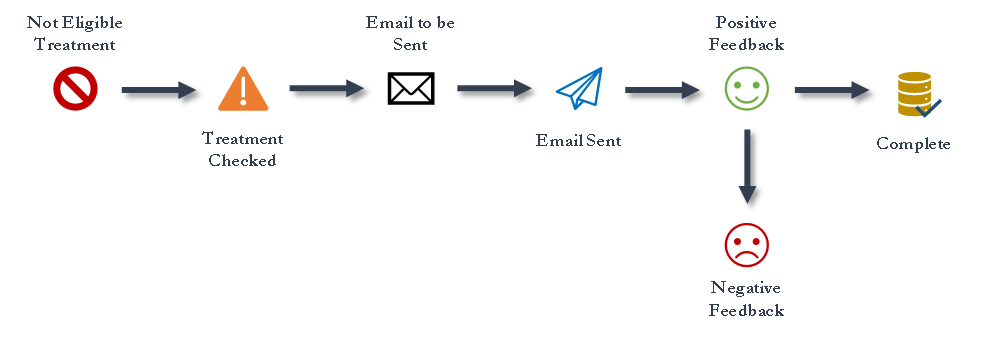
\includegraphics[width=1\linewidth]{Attachments/StatusTreatment} 

}

\caption{Flow of data collection status of treatments.}\label{fig:unnamed-chunk-1}
\end{figure}

\hypertarget{treatment.csv}{%
\subsection{Treatment.csv}\label{treatment.csv}}

List of data at treatment level with information and average/variance
index calculated.

\hypertarget{study-identifiers}{%
\subsubsection{Study identifiers:}\label{study-identifiers}}

\begin{itemize}
\tightlist
\item
  PaperID, TreatmentCode, n\_Paper, TreatmentName\_paper, Year, Outlet,
  Published \textasciitilde{} see
  \protect\hyperlink{Study_identifiers}{Social Norms meta.xlsx}
\end{itemize}

\hypertarget{design-variables-1}{%
\subsubsection{Design Variables:}\label{design-variables-1}}

\begin{itemize}
\tightlist
\item
  FirstTask, between\_vs\_within, Game\_type, Standard\_game,
  Group\_size, One\_Shot\_Repeated, Choice\_Method, Matching, Rounds,
  Punishment, Rewards, Monetary\_Incentivized\_experiment, Environment,
  Method\_elicitation, Separate\_sample\_beliefs, Belief\_repeated,
  Before\_after\_main\_decisions, KW\_Normative, KW\_Personal,
  Bicchieri\_Empirical, Bicchieri\_Normative,
  Bicchieri\_Personal\_Beliefs, Bicchieri\_between, Incentives\_beliefs,
  StatusTreatment\_Roma \textasciitilde{} see
  \protect\hyperlink{Study_identifiers}{Social Norms meta.xlsx}
\end{itemize}

\hypertarget{computed-variables}{%
\subsubsection{Computed Variables:}\label{computed-variables}}

contains the variables needed for the following analyses

\begin{itemize}
\tightlist
\item
  \textbf{Avg\_coop}: average cooperation (it changes based on game
  type, e.g.~in dictator game is computed as ``amount sent/endowment''
  );
\item
  \textbf{Var\_coop}: variance of cooperation;
\item
  \textbf{Avg\_NE}: average normative expectation (it changes based on
  elicitation method, Krupka-Weber or Bicchieri-Xiao)
\item
  \textbf{Var\_NE}: variance of normative expectation;
\item
  \textbf{Sd\_Avg\_NE}: indicate the standard deviation of sums of
  elicitation method scores in the possible choices set
\end{itemize}

\[\sigma\left(max\left( \frac{\sum_{j=1}^{J}\theta_j}{N} \right),\ \theta_j = \sum_{i=1}^{N}\alpha_{i,j}, \ j\in\{1,...,J\}\right)\]

\begin{itemize}
\tightlist
\item
  \textbf{Avg\_EE}: average empirical expectation (for Bicchieri-Xiao
  elicitation method)
\item
  \textbf{Avg\_PNB}: average personal belief (it changes based on
  elicitation method, Krupka-Weber or Bicchieri-Xiao)
\item
  \textbf{Var\_EE}: variance of empirical expectation
\item
  \textbf{Var\_PNB}: variance of personal belief
\end{itemize}

\hypertarget{beliefs}{%
\subsection{Subjects\_beliefs.csv}\label{beliefs}}

\begin{itemize}
\tightlist
\item
  \textbf{paper\_id}: it is the same of ``PaperID'' in Social Norms
  meta.xlsx
\item
  \textbf{treatment\_id}: it represents the treatment unique
  identification code ( = paper\_id \_ TreatmentCode)
\item
  \textbf{subject\_id}: it represents the subject unique identification
  code ( = treatment\_id \_ ``norm'' \_ subject code in row data or
  progressive number if missing)
\item
  \textbf{gender}: 1 if male, 0 if female
\item
  \textbf{age}: if exist only born date, it is calculated on the paper
  publication year
\item
  \textbf{scenarios}: indicate the set of possible value in the choice
  task
\item
  \textbf{KW\_Normative}: indicate the KW score of normative expectation
\item
  \textbf{Game\_type}: \textasciitilde{} see
  \protect\hyperlink{Study_identifiers}{Social Norms meta.xlsx}
\item
  \textbf{KW\_Personal}: indicate the average of personal belief in the
  norm task (Only in Krupka-Weber elicitation method)
\item
  \textbf{Bicchieri\_Empirical}: indicate the average of empirical
  expectation in norm task (Only in Bicchieri-Xiao elicitation method)
\item
  \textbf{Bicchieri\_Normative}: indicate the average of normative
  expectation in norm task (Only in Bicchieri-Xiao elicitation method)
\item
  \textbf{Bicchieri\_Personal}: indicate the average of personal belief
  in norm task (Only in Bicchieri-Xiao elicitation method)
\item
  \textbf{Design}: ``within'' if the sample among choice and belief task
  is the same, ``between'' otherwise.
\end{itemize}

\hypertarget{subjects_choice.csv}{%
\subsection{Subjects\_choice.csv}\label{subjects_choice.csv}}

\begin{itemize}
\tightlist
\item
  subject\_id, treatment\_id, paper\_id, gender, age, Design,
  Game\_type, scenarios \textasciitilde{} see
  \protect\hyperlink{beliefs}{Subjects\_beliefs.csv}
\item
  \textbf{choice}: indicate the subject choice in the game (e.g.~in a
  dictator game indicate the amount of money/token that dictator sent to
  recipient)
\item
  \textbf{A}: 1 if choice is equal to scenario (by row), 0 otherwise
\item
  \textbf{endowment}: indicate initial endowment.
\end{itemize}

\hypertarget{method-clarification}{%
\section{Method Clarification}\label{method-clarification}}

\hypertarget{paper-search-and-feeding-papers-database}{%
\subsection{Paper search and feeding papers
database}\label{paper-search-and-feeding-papers-database}}

Thanks to different research platforms (Search Engine Platforms), as
Google Scholar, EconRepec, WebOfScience, Ideas and Google group ESA, we
find 165 paper about cooperation and elicitation of social norms
(corresponding to 452 treatments).

\hypertarget{search-criteria}{%
\subsection{Search criteria}\label{search-criteria}}

The selection criteria to identify papers in target was:

\begin{itemize}
\tightlist
\item
  \textbf{Game type} (cooperation and prosociality games):

  \begin{itemize}
  \tightlist
  \item
    Dictator Game (with tax/standard/Lying);
  \item
    Donation Game;
  \item
    Ultimatum Game;
  \item
    Trust Game;
  \item
    Public Good Game;
  \item
    Prisoner's Dilemma Game;
  \item
    Take or Give Fame;
  \item
    CPR;
  \item
    Bargaining Game;
  \item
    Tax Game;
  \item
    Investment Game;
  \end{itemize}
\item
  Presence of norm elicitation task:

  \begin{itemize}
  \tightlist
  \item
    Krupka and Weber (2013);
  \item
    Bicchieri-Xiao (2009).
  \end{itemize}
\item
  Only monetary incentivized studies (both choices and norms
  elicitation).
\end{itemize}

\begin{table}

\caption{\label{tab:unnamed-chunk-2}Summary of Major Variables per Game Type}
\begin{tabular}[t]{>{}lccccccc}
\toprule
Game type & Treatment per Game Type & Between Subjects Beliefs & KW & Bicchieri & KW and Bicchieri & Only Norms & Available Data\\
\midrule
\textbf{DG} & 108 & 42 & 69 & 31 & 8 & 1 & 36\\
\textbf{PGG} & 30 & 18 & 23 & 2 & 2 & 0 & 17\\
\textbf{UG} & 20 & 18 & 8 & 12 & 0 & 0 & 3\\
\textbf{TG} & 11 & 7 & 7 & 4 & 0 & 0 & 5\\
\textbf{PDG} & 8 & 2 & 2 & 6 & 0 & 0 & 0\\
\addlinespace
\textbf{Donation Game} & 7 & 4 & 7 & 0 & 0 & 0 & 5\\
\textbf{Tax Game} & 7 & 0 & 1 & 0 & 6 & 0 & 0\\
\textbf{ToG} & 7 & 7 & 7 & 0 & 0 & 0 & 3\\
\textbf{CPR} & 5 & 0 & 0 & 5 & 0 & 0 & 0\\
\textbf{GEG} & 5 & 3 & 5 & 0 & 0 & 0 & 5\\
\addlinespace
\textbf{DG Tax} & 2 & 0 & 2 & 0 & 0 & 0 & 2\\
\textbf{BG} & 1 & 0 & 1 & 0 & 0 & 0 & 1\\
\textbf{Lying DG} & 1 & 0 & 1 & 0 & 0 & 0 & 1\\
\textbf{Third-Party Lying DG} & 1 & 0 & 1 & 0 & 0 & 0 & 1\\
\bottomrule
\end{tabular}
\end{table}

Thanks to different research platforms (Search Engine Platforms), as
Google Scholar, EconRepec, WebOfScience, Ideas and Google group ESA, we
find 165 paper about cooperation and elicitation of social norms
(corresponding to 452 treatments).

Following these criteria, the number of treatments in target is 213.

\hypertarget{homogeneity-criteria}{%
\section{Homogeneity Criteria}\label{homogeneity-criteria}}

For all games, we take into consideration the first round observation
and the allocation where dictator have the maximum endowment and
recipient have zero.

\hypertarget{dictator-game-dg}{%
\subsection{Dictator Game (DG)}\label{dictator-game-dg}}

We consider all DGs including at least two or more real players (no
computers).

\hypertarget{choice-data}{%
\subsubsection{Choice data:}\label{choice-data}}

\begin{itemize}
\tightlist
\item
  In case of repeated rounds, we consider only first-round decisions; if
  stranger matching protocol, and rounds differ in any of the design
  features (e.g., endowment, number of players, etc.) we can consider
  these as single independent observations
\item
  To define cooperation levels, we look at final allocations; hence, for
  example, if dictators have some restrictions applying on their
  choices, such as donating only part of his endowment, we consider as
  cooperation the ratio between amount sent and total endowment
\item
  No minigames (if minigames, these are flagged and possibly used in
  future analyses)
\end{itemize}

\hypertarget{norm-data}{%
\subsubsection{Norm data:}\label{norm-data}}

\begin{itemize}
\tightlist
\item
  If KW: norm (normative expectation) is computed by summing
  appropriateness scores of each actions and selecting the action with
  highest score; variance of norm is defined by computing the variance
  of appropriateness scores;
\item
  If Bicchieri: average norm (normative expectation) is computed as
  average of subjects' answers; we compute the variance of a norm by
  computing the variance of scores;
\item
  If elicitation within subjects, only norm elicited from subjects
  playing role of Dictators;
\item
  If elicited actions are a subset of choice actions, then we considered
  the paper anyway
\end{itemize}

\hypertarget{criteria-for-being-defined-as-standard-ref.-engel-2011}{%
\subsubsection{Criteria for being defined as ``Standard'' (ref. Engel
2011)}\label{criteria-for-being-defined-as-standard-ref.-engel-2011}}

\begin{itemize}
\tightlist
\item
  Not a minigame
\item
  Two players
\item
  No papers that give the recipient any kind of power (and thereby bring
  the experiment close to an ultimatum game);
\item
  No papers that mix the motive of benevolence with one of sanctioning
  the recipient
\item
  No papers that limit the dictator's action space such that it does not
  include the option to give nothing nor to take from the recipient
\item
  No real effort task used to determine the dictator's endowment
\end{itemize}

\hypertarget{take-or-give-game-tog}{%
\subsection{Take or Give Game (ToG)}\label{take-or-give-game-tog}}

This category includes DG with take framing.

\begin{itemize}
\tightlist
\item
  To define cooperation levels, we look at final allocations; hence, for
  example, if dictators have some restrictions applying on their
  choices, such as donating only part of his endowment, we consider as
  cooperation the ratio between amount sent and total endowment.
\end{itemize}

\hypertarget{public-good-game-pgg}{%
\subsection{Public Good Game (PGG)}\label{public-good-game-pgg}}

Lorem ipsum dolor sit amet, consectetuer adipiscing elit. Maecenas
porttitor congue massa. Fusce posuere, magna sed pulvinar ultricies,
purus lectus malesuada libero, sit amet commodo magna eros quis urna.
Nunc viverra imperdiet enim. Fusce est. Vivamus a tellus. Pellentesque
habitant morbi tristique senectus et netus et malesuada fames ac turpis
egestas. Proin pharetra nonummy pede. Mauris et orci.

\end{document}
